\chapter{Überschreiben}

\section*{Lösung}

\begin{itemize}
    \item void f(int i)
\end{itemize}


\section*{Anmerkungen und Ergänzungen}

\textbf{Überschreiben} und \textbf{Überladen} sind zwei unterschiedliche Konzepte\footnote{Seite 210 im Skript}:

\begin{itemize}
    \item Eine Methode wird in einer Unterklasse \textit{überschrieben}, wenn Name, Signatur und Rückgabetyp der Methode der Unterklasse mit der
    Methode der Oberklasse übereinstimmen.
    \item Eine Methode wird \textit{überladen}, wenn eine Methode mit gleichem Namen bereitgestellt wird, aber eine unterschiedliche Signatur
    aufweist.
    Der Rückgabetyp darf abweichen:
    \blockquote[Java Language Specification - 8.4.9. Overloading\footnote{\url{https://docs.oracle.com/javase/specs/jls/se21/html/jls-8.html#jls-8.4.9}}]{
        There is no required relationship between the return types or between the throws clauses of two methods with the same name, unless their signatures are override-equivalent.
    }
\end{itemize}

\subsection*{Exkurs - Kovarianz}
Sobald es sich bei dem Rückgabetyp einer Methode um einen \textit{Referenztypen} handelt, muß der Rückgabetyp der Methode in der Unterklasse
folgende Bedingung erfüllen\footnote{
vgl. ``Java Language Specification - 8.4.8.3. Requirements in Overriding and Hiding``: \url{https://docs.oracle.com/javase/specs/jls/se21/html/jls-8.html#jls-8.4.8.3}
}:

\begin{itemize}
    \item Der Rückgabetyp der Methode in der Unterklasse muss \textbf{kovariant} zu dem Rückgabetyp der überschriebenen Methode sein\footnote{
        vgl. ``Java Language Specification - 8.4.5. Method Result``: \url{https://docs.oracle.com/javase/specs/jls/se21/html/jls-8.html#jls-8.4.5}
    }
\end{itemize}

Kovariant bedeutet, dass der Rückgabetyp in der Methode der Unterklasse nicht allgemeiner sein darf als der Rückgabetyp der Methode der Oberklasse:
Sowohl Richtung der Vererbungshierarchie der als auch die Richtung der Typhierarchie stimmen überein:

\begin{itemize}
    \item Unterklasse $\leftarrow$ Oberklasse\footnote{
        ``$\leftarrow$``: Richtung d. Vererbungshierarchie
    }
    \item Rückgabetyp Methode Unterklasse $\leftarrow$ Rückgabetyp Methode Oberklasse\footnote{
        ``$\leftarrow$``: Richtung d. Typhierarchie
    }
\end{itemize}

Zur Verdeutlichung können die in dem Kurs bereits verwendeten geometrischen Figuren betrachtet werden:

\begin{figure}[h]
    \centering
    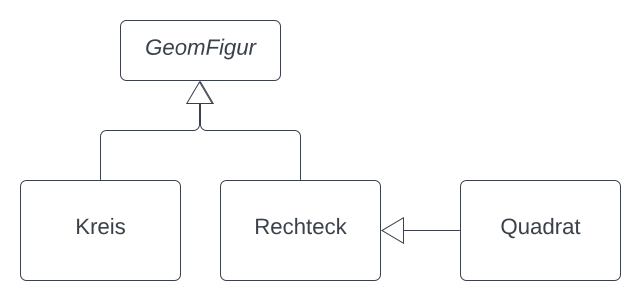
\includegraphics[
        width=8cm,
        keepaspectratio,
    ]{chapters/1. Überschreiben/img/figur}
    \caption{Vererbungshierarchie der Klasse \textit{GeomFigur} und ihrer Subklassen.}
    \label{fig:figur}
\end{figure}

Eine Klasse \code{FigurenFabrik} sei folgendermaßen gegeben:

\begin{lstlisting}[language=java]

class FigurenFabrik {

    /**
     * Erzeugt ein neues Quadrat mit der spezifizierten Seitenlänge.
     *
     * @param seitenLaenge die spezifizierte Seitenlänge.
     */
    public Quadrat erzeugeQuadrat(double seitenLaenge) {
        return new Quadrat(seitenLaenge);
    }
}
\end{lstlisting}

Eine Klasse, die von \code{FigurenFarik} erbt und \code{erzeugeQuadrat} überschreiben möchte,
muss sicherstellen, dass das von der Methode zurückgelieferte Objekt auch tatsächlich ein \code{Quadrat} ist.

Hierzu darf der Rückgabetyp nicht allgemeiner sein. `Allgemeiner` bedeutet in diesem Fall: Typ \code{Rechteck} oder \code{Figur}.

Ansonsten würden Zugriffe auf (vererbbare) spezifische Eigenschaften der Klasse \code{Quadrat} mit den zurückgelieferten Objekten zu Fehlern führen.
Der Compiler verhindert dies bereits:

\begin{lstlisting}[language=java]
class KaputteFigurenFabrik extends FigurenFabrik {

    public Rechteck erzeugeQuadrat(double seitenLaenge) {
        return new Rechteck(seitenLaenge, seitenLaenge*2);
    }
}

public class FigurenMacher {

    public static void main(String[] args) {
        FigurenFabrik f = new FigurenFabrik();

        // bevor es zum Programmabsturz waehrend der Laufzeit
        // aufgrund eines Aufrufs einer nur in Quadrat bekannten
        // Methode kommt, bricht der Compiler den Uebersetzungsvorgang
        // bereits mit einem Fehler ab
        f.erzeugeQuadrat().spezifischeMethodeAusQuadrat();
    }

}
\end{lstlisting}

Der vom Compiler ausgegebene Fehler weist auf die Inkompatibilität der Rückgabetypen hin:

\begin{lstlisting}[language=text]
return type Rechteck is not compatible with Quadrat.
\end{lstlisting}

Für \textbf{Kovarianz} (und in diesem Zusammenhang \textbf{Kontravarianz}) und formalere Herleitungen sei auf
\textit{Das Liskovsche Substitutionsprinzip}\footnote{``Wikipedia - Liskov substitution principle``: \url{https://en.wikipedia.org/wiki/Liskov_substitution_principle}} (\cite{Lis87})
sowie den ausführlichen Beitrag im englischsprachigen Wikipedia \footnote{
    ``Wikipedia - Covariance and Contravariance``: \url{https://en.wikipedia.org/wiki/Covariance_and_contravariance_(computer_science)}
} verwiesen.
